%für Sprache, A4 Blatt, float, Grafiken, UTF Codierung, PDF, Color, Seitenabstand, Listings
\documentclass[a4papr,12pt]{article}
\usepackage[utf8]{inputenc}
\usepackage[ngerman]{babel}
\usepackage{graphicx}
\usepackage{float}
\usepackage{textcomp}
\usepackage{pdfpages}
\usepackage{tikz}
\usepackage{hyperref}
\usepackage{geometry}
\usepackage{listings}
\usepackage{color}
\usepackage{grffile}
\usepackage{caption}

%Mathematics
\usepackage{amstext}
\usepackage{amssymb}
\usepackage{amsmath}
\usepackage{amsfonts}
\usepackage{mathrsfs}
\usepackage{mathtools}

%include this before fancy or page style gets messed up bc of geometry
%Seitenabstand A4 Blatt
\geometry{a4paper}
\geometry{top=25mm,bottom=25mm,left=23mm,right=20mm}

% macro to select a scaled-down version of Bera Mono (for instance)
\makeatletter
\newcommand\BeraMonottfamily{%
  \def\fvm@Scale{0.85}% scales the font down
  \fontfamily{fvm}\selectfont% selects the Bera Mono font
}
\makeatother

%Hyperref zum anklicken von Überschriften in Texmaker + Farben einstellen
\hypersetup{
	colorlinks,
	citecolor=black,
	filecolor=black,
	linkcolor=blue,
	urlcolor=black
}

\definecolor{mygreen}{rgb}{0,0.6,0}
\definecolor{mygray}{rgb}{0.5,0.5,0.5}
\definecolor{mymauve}{rgb}{0.58,0,0.82}

%Zum Pascal Code einfügen mit lstinputlisting[language=Pascal] {../blabla.pas}
\lstset{ %
  backgroundcolor=\color{white},   % choose the background color; you must add \usepackage{color} or 								  \usepackage{xcolor}
  basicstyle=\BeraMonottfamily,        % the size of the fonts that are used for the code
  breakatwhitespace=false,         % sets if automatic breaks should only happen at whitespace
  breaklines=true,                 % sets automatic line breaking
  captionpos=b,                    % sets the caption-position to bottom
  commentstyle=\color{mygreen},    % comment style
  deletekeywords={...},            % if you want to delete keywords from the given language
  escapeinside={\%*}{*)},          % if you want to add LaTeX within your code
  extendedchars=true,              % lets you use non-ASCII characters; for 8-bits encodings only, 												does not work with UTF-8
  frame=single,	               % adds a frame around the code
  keepspaces=true,                 % keeps spaces in text, useful for keeping indentation of code 									  (possibly needs columns=flexible)
  keywordstyle=\color{blue},       % keyword style
  language=Octave,                 % the language of the code
  otherkeywords={...},           % if you want to add more keywords to the set
  numbers=left,                    % where to put the line-numbers; possible values are (none, left, 								  right)
  numbersep=5pt,                   % how far the line-numbers are from the code
  numberstyle=\tiny\color{black}, % the style that is used for the line-numbers
  rulecolor=\color{black},         % if not set, the frame-color may be changed on line-breaks within 								  not-black text (e.g. comments (green here))
  showspaces=false,                % show spaces everywhere adding particular underscores; it 														overrides 'showstringspaces'
  showstringspaces=false,          % underline spaces within strings only
  showtabs=false,                  % show tabs within strings adding particular underscores
  stepnumber=2,                    % the step between two line-numbers. If it's 1, each line will be 								  numbered
  stringstyle=\color{mymauve},     % string literal style
  title=\getlstname,
  tabsize=2,	                    % sets default tabsize to 2 spaces
  inputencoding=latin1,
  columns=fullflexible
}

\lstset{literate=%
	{Ö}{{\"O}}1
	{Ä}{{\"A}}1
	{Ü}{{\"U}}1
	{ß}{{\ss}}1
	{ü}{{\"u}}1
	{ä}{{\"a}}1
	{ö}{{\"o}}1
	{~}{{\textasciitilde}}1
}

%Filenamen und Pfad trennen
\makeatletter
\DeclareRobustCommand{\getlstname}{%
\begingroup
  % \lstname seems to change hyphens into \textendash
  \def\textendash{-}%
  \filename@parse{\lstname}%
  \texttt{\filename@base.\filename@ext}%
\endgroup
}


%Für Kopfzeile den Style
\usepackage{fancyhdr}
\pagestyle{fancy}
\lhead{AUD 2\textbackslash PRO 2 - Übung 3}
\rhead{Andreas Roither, \today{}}
\newcommand{\Cross}{\mathbin{\tikz [x=1.4ex,y=1.4ex,line width=.2ex] \draw (0,0) -- (1,1) (0,1) -- (1,0);}}%

\begin{document}

%ANGABE     
\thispagestyle{plain}
\includepdf[pages={1},pagecommand={     
\begin{tikzpicture}[remember picture, overlay]\node at (15.8, -0.85) {6 h};\end{tikzpicture}
\begin{tikzpicture}[remember picture, overlay]\node at (7.6, -0.85) {Andreas Roither};\end{tikzpicture}
\begin{Huge}
\begin{tikzpicture}[remember picture, overlay]\node at (-1.3, -1.9) {X};\end{tikzpicture}
\end{Huge}
}]{Angabe/UE3.pdf}
\thispagestyle{plain}
\includepdf[pages=2-,pagecommand={}]{Angabe/UE3.pdf}

\section*{Übung 3}
\subsection*{Aufgabe 1}
\subsubsection*{Lösungsidee}
Bei der Dekompression und der Kompression wird Zeichen für Zeichen überprüft ob es eine Nummer oder ein anderer Charakter ist. Falls eine Nummer bei der Dekompression  vorkommt, wird das vorherige Zeichen dementsprechend oft eingefügt. Bei der Kompression wird die Anzahl des nacheinander auftretenden Buchstabens gezählt und mit dem Buchstaben in die txt Datei geschrieben. Bei der Kompression und anschließender Dekompression kann eine Zahl bei Sonderkombinationen zu einem falschen Ergebnis führen. Bsp: \grqq{}aaaa1\grqq{} würde bei einer Umwandlung \grqq{}a41\grqq{} werden. Bei anschließender Dekompression werden jedoch daraus 41 a und nicht wie vorher 4 a Zeichen.
\newline

\lstinputlisting[language=Pascal] {../rle.pas}
\begin{figure}[H]
	\centering
	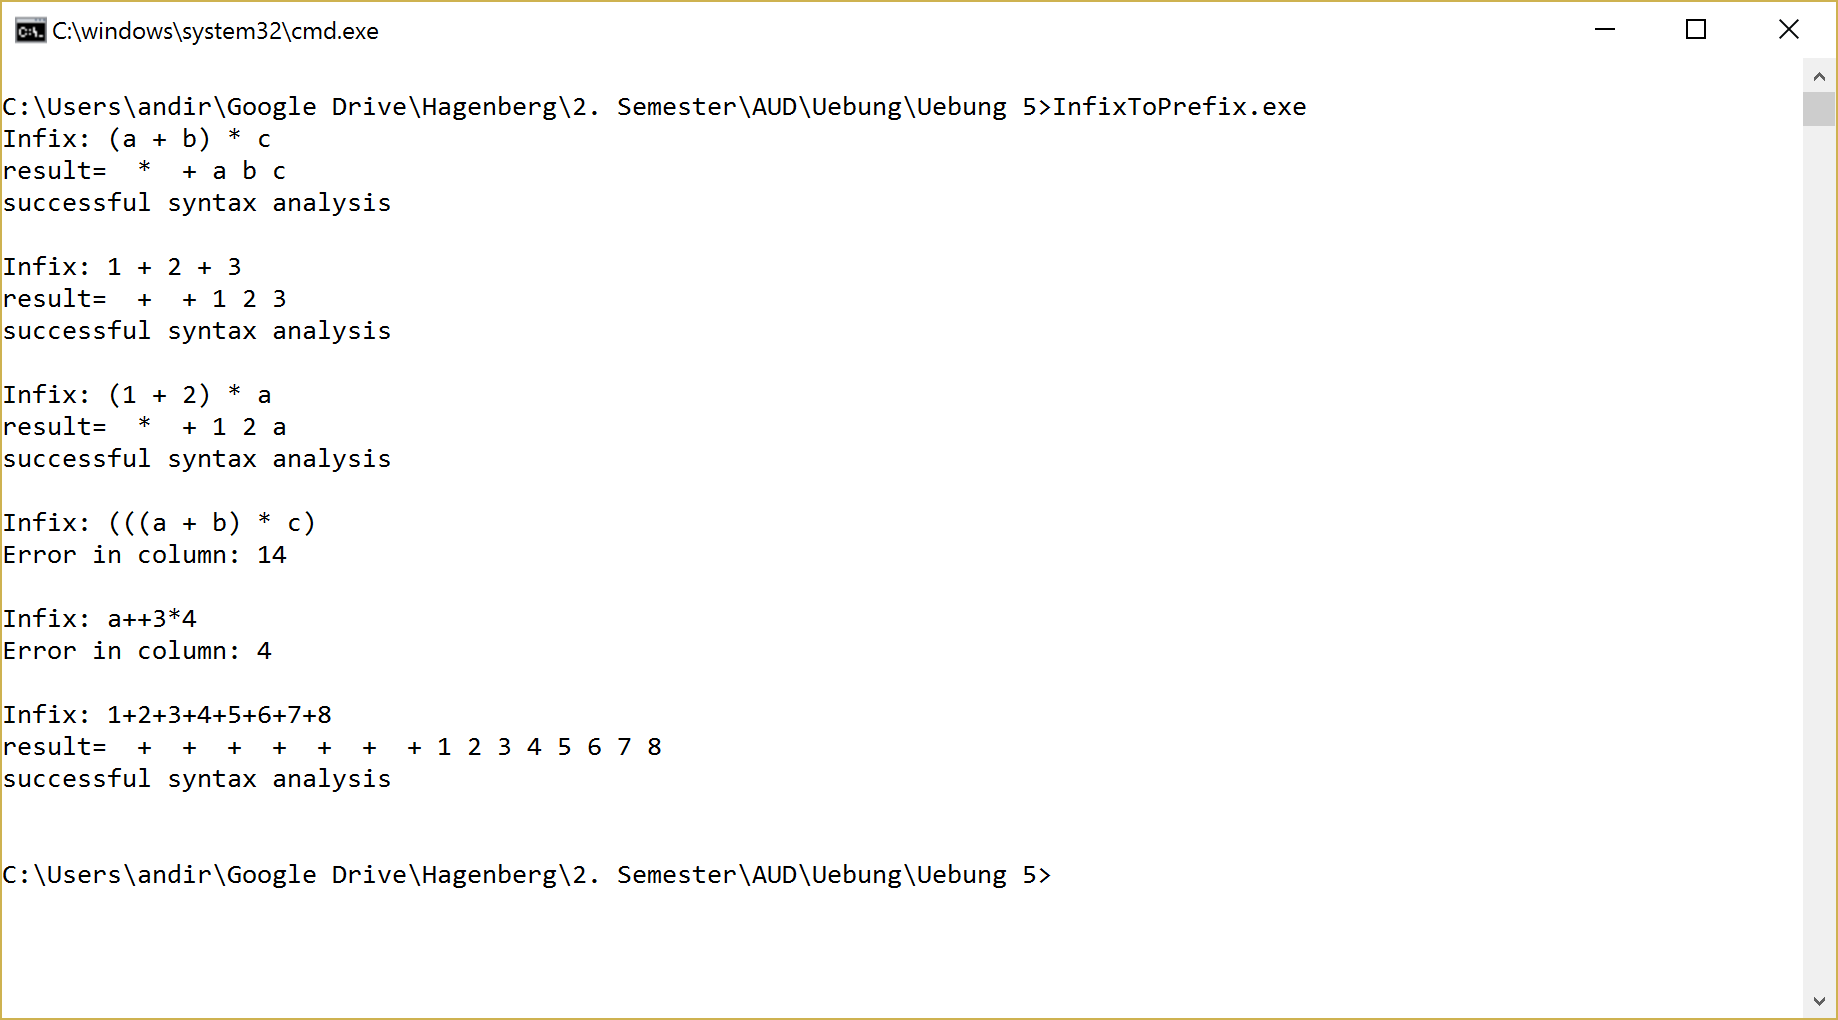
\includegraphics[scale=0.75]{./pictures/1.png}
	\caption{RLE Optionen}
	\label{fig: Options}
\end{figure}
Zu sehen sind die zwei verschiedenen Optionen und die Eingabeaufforderung falls nichts angegeben wurde.\newline

\lstinputlisting[language=] {../d.txt}
\lstinputlisting[language=] {../c.txt}

In d.txt ist der dekomprimierte Text, in c.txt der komprimierte.

\newpage
\subsection*{Aufgabe 2}
\subsubsection*{Lösungsidee}
Zuerst werden die Wörter die ersetzt werden sollen eingelesen und in einer Hash Tabelle gespeichert. Jedes Zeichen in der Ostern.txt wird eingelesen und vorkommende Wörter werden überprüft. Der berechnete Hashwert eines Wortes wird mit einem Element in der Hash Tabelle an der Position des Hashwertes verglichen. Falls ein Element mit dem Hashcode existiert und genau dasselbe Wort ist (Vergleich, falls ein Wort mit dem selben Hashwert existiert jedoch nicht Zeichen für Zeichen gleich ist), wird das ersetzende Wort in die neue txt Datei eingefügt, andernfalls wird das ursprüngliche Wort eingefügt.   
\newline

\lstinputlisting[language=Pascal] {../storygen.pas}
\begin{figure}[H]
	\centering
	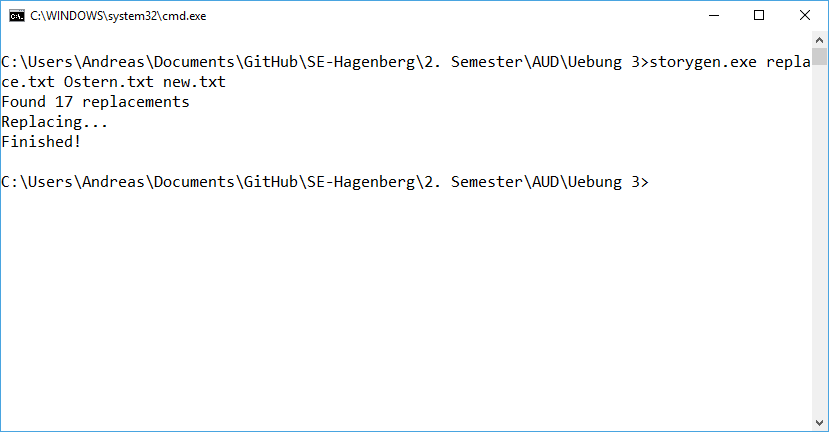
\includegraphics[scale=0.75]{./pictures/2.png}
	\caption{Storygen}
	\label{fig: Matching}
\end{figure}
\newpage
\lstinputlisting[] {../replace.txt}
\raggedright
In der replace.txt werden die Wörter die ersetzt werden sollen und die Wörter durch die sie ersetzt werden sollen gespeichert, getrennt durch ein beliebiges Trennzeichen (außer Buchstaben).
\newline

\lstinputlisting[linerange={1-8}] {../Ostern.txt}
\lstinputlisting[linerange={1-8}] {../new.txt}
\raggedright
Zu sehen sind die ersten 8 Zeilen der Ostern.txt und der new.txt. Wörter, die in der replace.txt vorgegeben sind, wie Osterhasen oder Hühnchen wurden durch die in der replace.txt vorhandenen Wörtern ersetzt.

\end{document}





